\documentclass[11pt,a4paper,twoside]{article}

% Deutsche Spracheinstellungen
\usepackage[english,english]{babel, varioref}
\usepackage[T1]{fontenc}
\usepackage[utf8]{inputenc}

%\usepackage{marvosym}

\usepackage{amsfonts}
\usepackage{amssymb}
\usepackage{amsmath}
\usepackage{amscd}
\usepackage{amstext}
\usepackage{float}
\usepackage{caption}
\usepackage{wrapfig}
\usepackage{setspace}
%\usepackage[onehalfspacing]{setspace}
\usepackage{threeparttable}
\usepackage{footnote}
\usepackage{feynmf}
\usepackage{bbm}
\usepackage{slashed}
\usepackage{textcomp}
\usepackage{multirow}
\usepackage{courier}
\usepackage{listings}
\usepackage{color}
%\usepackage{minipage}
 
 \definecolor{middlegray}{rgb}{0.5,0.5,0.5}
 \definecolor{lightgray}{rgb}{0.8,0.8,0.8}
 \definecolor{orange}{rgb}{0.8,0.3,0.3}
 \definecolor{yac}{rgb}{0.6,0.6,0.1}
 \definecolor{puple}{rgb}{0.62,0.12,0.94}
 \lstset{language=Python,
                basicstyle=\ttfamily,
                keywordstyle=\color{red}\ttfamily,
                stringstyle=\color{magenta}\ttfamily,
                commentstyle=\color{blue}\ttfamily,
                morecomment=[l][\color{blue}]{\#},
		%stepnumber=1,
		%numberstyle=\color{magenta}\ttfamily,
		%    numbers=left,
		%    numberstyle={},
		%    numberblanklines=false,
		%    stepnumber=1,
		%    numbersep=10pt,
		    xleftmargin=15pt,
 		moredelim=[is][\color{purple}]{|}{|}
}

\newfloat{formel}{htbp}{for}
\floatname{formel}{Formel}

\onehalfspacing
%\setstretch {1.433}

\usepackage{longtable}

%\usepackage{bibgerm}

\usepackage{footnpag}

\usepackage{ifthen}                 %%% package for conditionals in TeX
\usepackage[amssymb]{SIunits}
%Fr textumflossene Bilder und Tablellen
%\usepackage{floatflt} - veraltet

%Fr Testzwecke aktivieren, zeigt labels und refs im Text an.
%\usepackage{showkeys}

% Abstand zwischen zwei Abs�zen nach DIN (1,5 Zeilen)
% \setlength{\parskip}{1.5ex}

% Einrckung am Anfang eines neuen Absatzes nach DIN (keine)
%\setlength{\parindent}{0pt}

% R�der definieren
% \setlength{\oddsidemargin}{0.3cm}
% \setlength{\textwidth}{15.6cm}

% bessere Bildunterschriften
\usepackage{caption2}


% Probleml�ungen beim Umgang mit Gleitumgebungen
\usepackage{float}

% Nummeriert bis zur Strukturstufe 3 (also <section>, <subsection> und <subsubsection>)
%\setcounter{secnumdepth}{3}

% Fhrt das Inhaltsverzeichnis bis zur Strukturstufe 3
%\setcounter{tocdepth}{3}

\usepackage{exscale}

\newenvironment{dsm} {\begin{displaymath}} {\end{displaymath}}
\newenvironment{vars} {\begin{center}\scriptsize} {\normalsize \end{center}}


\newcommand {\en} {\varepsilon_0}               % Epsilon-Null aus der Elektrodynamik
\newcommand {\lap} {\; \mathbf{\Delta}}         % Laplace-Operator
\newcommand {\R} { \mathbb{R} }                 % Menge der reellen Zahlen
\newcommand {\e} { \ \mathbf{e} }               % Eulersche Zahl
\renewcommand {\i} { \mathbf{i} }               % komplexe Zahl i
\newcommand {\N} { \mathbb{N} }                 % Menge der nat. Zahlen
\newcommand {\C} { \mathbb{C} }                 % Menge der kompl. Zahlen
\newcommand {\Z} { \mathbb{Z} }                 % Menge der kompl. Zahlen
\newcommand {\limi}[1]{\lim_{#1 \rightarrow \infty}} % Limes unendlich
\newcommand {\sumi}[1]{\sum_{#1=0}^\infty}
\newcommand {\rot} {\; \mathrm{rot} \,}         % Rotation
\newcommand {\grad} {\; \mathrm{grad} \,}       % Gradient
\newcommand {\dive} {\; \mathrm{div} \,}        % Divergenz
\newcommand {\dx} {\; \mathrm{d} }              % Differential d
\newcommand {\cotanh} {\; \mathrm{cotanh} \,}   %Cotangenshyperbolicus
\newcommand {\asinh} {\; \mathrm{areasinh} \,}  %Area-Sinus-Hyp.
\newcommand {\acosh} {\; \mathrm{areacosh} \,}  %Area-Cosinus-H.
\newcommand {\atanh} {\; \mathrm{areatanh} \,}  %Area Tangens-H.
\newcommand {\acoth} {\; \mathrm{areacoth} \,}  % Area-cotangens
\newcommand {\Sp} {\; \mathrm{Sp} \,}
\newcommand {\mbe} {\stackrel{\text{!}}{=}}     %Must Be Equal
\newcommand{\qed} { \hfill $\square$\\}
\newcommand{\midtilde}{\raisebox{-0,25\baselineskip}{\textasciitilde}}
\renewcommand{\i} {\imath}
\def\captionsngerman{\def\figurename{\textbf{Abb.}}}

%%%%%%%%%%%%%%%%%%%%%%%%%%%%%%%%%%%%%%%%%%%%%%%%%%%%%%%%%%%%%%%%%%%%%%%%%%%%
% SWITCH FOR PDFLATEX or LATEX
%%%%%%%%%%%%%%%%%%%%%%%%%%%%%%%%%%%%%%%%%%%%%%%%%%%%%%%%%%%%%%%%%%%%%%%%%%%%
%%%
\ifx\pdfoutput\undefined %%%%%%%%%%%%%%%%%%%%%%%%%%%%%%%%%%%%%%%%% LATEX %%%
%%%
\usepackage[dvips]{graphicx}       %%% graphics for dvips
\DeclareGraphicsExtensions{.eps,.ps}   %%% standard extension for included graphics
\usepackage[ps2pdf]{thumbpdf}      %%% thumbnails for ps2pdf
\usepackage[ps2pdf,                %%% hyper-references for ps2pdf
bookmarks=true,%                   %%% generate bookmarks ...
bookmarksnumbered=true,%           %%% ... with numbers
hypertexnames=false,%              %%% needed for correct links to figures !!!
breaklinks=true,%                  %%% breaks lines, but links are very small
linkbordercolor={0 0 1},%          %%% blue frames around links
pdfborder={0 0 112.0}]{hyperref}%  %%% border-width of frames
%                                      will be multiplied with 0.009 by ps2pdf
%
\hypersetup{ pdfauthor   = {Dimitrios Skodras},
pdftitle    = {Fermionic Dark Matter and its Role on B Anomalies}, pdfsubject  = {masterthesis}, pdfkeywords = {dark matter},
pdfcreator  = {LaTeX with hyperref package}, pdfproducer = {dvips
+ ps2pdf} }
%%%
\else %%%%%%%%%%%%%%%%%%%%%%%%%%%%%%%%%%%%%%%%%%%%%%%%%%%%%%%%%% PDFLATEX %%%
%%%
\usepackage[pdftex]{graphicx}      %%% graphics for pdfLaTeX
\DeclareGraphicsExtensions{.pdf}   %%% standard extension for included graphics
\usepackage[pdftex]{thumbpdf}      %%% thumbnails for pdflatex
\usepackage[pdftex,                %%% hyper-references for pdflatex
bookmarks=true,%                   %%% generate bookmarks ...
bookmarksnumbered=true,%           %%% ... with numbers
hypertexnames=false,%              %%% needed for correct links to figures !!!
breaklinks=true,%                  %%% break links if exceeding a single line
linkbordercolor={0 0 1},
linktocpage]{hyperref} %%% blue frames around links
%                                  %%% pdfborder={0 0 1} is the default
\hypersetup{
pdftitle    = {Fermionic Dark Matter and its Role on B Anomalies}, %right place
pdfsubject  = {master thesis}, 
pdfkeywords = {V301, Innenwiderstand, Leistungsanpassung},
pdfsubject  = {Protokoll AP},
pdfkeywords = {V301, Innenwiderstand, Leistungsanpassung}}
%                                  %%% pdfcreator, pdfproducer,
%                                      and CreationDate are automatically set
%                                      by pdflatex !!!
\pdfadjustspacing=1                %%% force LaTeX-like character spacing
\usepackage{epstopdf}
%
\fi %%%%%%%%%%%%%%%%%%%%%%%%%%%%%%%%%%%%%%%%%%%%%%%%%%% END OF CONDITION %%%
%%%%%%%%%%%%%%%%%%%%%%%%%%%%%%%%%%%%%%%%%%%%%%%%%%%%%%%%%%%%%%%%%%%%%%%%%%%%
% seitliche Tabellen und Abbildungen
%\usepackage{rotating}
\usepackage{ae}
\usepackage{
  array,
  booktabs,
  dcolumn
}
\makeatletter 
  \renewenvironment{figure}[1][] {% 
    \ifthenelse{\equal{#1}{}}{% 
      \@float{figure} 
    }{% 
      \@float{figure}[#1]% 
    }% 
    \centering 
  }{% 
    \end@float 
  } 
  \makeatother 


  \makeatletter 
  \renewenvironment{table}[1][] {% 
    \ifthenelse{\equal{#1}{}}{% 
      \@float{table} 
    }{% 
      \@float{table}[#1]% 
    }% 
    \centering 
  }{% 
    \end@float 
  } 
  \makeatother 
%\usepackage{listings}
%\lstloadlanguages{[Visual]Basic}
%\allowdisplaybreaks[1]
%\usepackage{hycap}
%\usepackage{fancyunits}

\usepackage{xfrac}
\usepackage{xcolor}
\usepackage{setspace}\usepackage{threeparttable}
\usepackage{fancyhdr}
\fancyfoot{}
\fancyhead[RO,LE]{\thepage}
\fancyhead[LO]{\leftmark}
\fancyhead[RE]{\rightmark}


 %\setlength{\parskip}{1.5ex}
\begin{document}
\begin{spacing}{1,2}
\pagenumbering{Roman}

% Anmerkung: Die Seitenraender wurden asymmetrisch gewaehlt,
%            damit genug Platz fuer eine Klemmbindung da ist.
%            Da neue Kapitel auf der rechten Seite (ungerade
%            Seitennummer) beginnen sollten, muss ggf. am Ende
%            des vorhergehenden Kapitels eine Leerseite
%            eingefuegt werden:
%
%            \newpage
%            \thispagestyle{empty}
%            \ \\
%            \newpage
%
%            Die Seitenraender koennen aber auch in der Datei Tex/global.tex
%            veraendert werden.

% >>> Titelseite <<<

\newcommand{\thetitle}{DM sheds light (up)on flavor anomalies}

\thispagestyle{empty}
\begin{center}

\Huge\textbf{\thetitle}
\vfill
% Note that the size is given in normal parentheses
% instead of curly brackets.
% Define external vertices from bottom to top
\vfill

\end{center}
\newpage
% % >>> Gutachterseite <<<
% \thispagestyle{empty}
% \newpage
% \cleardoublepage




% >>> Kurzfassung/Abstract <<<


% >>> Hauptteil <<<

%\addcontentsline{toc}{chapter}{Inhaltsverzeichnis}


\pagenumbering{arabic}
\setcounter{page}{1}

\section{Model outline}

\begin{table}
 \begin{tabular}{c|c|c|c}
  Field & $SU(3)_C\times SU(2)_L\times U(1)_{Y_W}$ & $A_4 \times U(1)_\text{FN} \times Z_3$ & $U(1)_\chi$\\
  \hline
  $Q^i_L$ & (3,2,$\frac16$) & (1,$a^i$,$\omega$) & 0\\
  $U^i_R$ & (3,1,$\frac23$) & (1,$b^i$,$\omega^2$)& 0\\
  $D^i_R$ & (3,1,$-\frac13$) & (1,$c^i$,$\omega^2$)& 0\\
  $L^i_L$ & (1,2,$-\frac12$) & (3,0,$\omega$)& 0\\
  $E^i_R$ & (1,1,$-1$) & ($1 {^(} {'} {^,} '' {^)} $,$d^i$,$\omega^2$)& 0\\
  $\Phi_H$ & (1,2,$\frac12$) & (1,0,1)& 0\\
  \hline
  $\psi$ & (1,1,0) & (1,0,$\omega^2$)& 1\\
  $\Phi_l$ & (1,2,-$\frac12$) & ($1''$,0,1)& 1\\
  $\Phi_q$ & (3,2,$\frac16$) & ($1$,0,1)& 1\\
  \hline
  $\Phi_T$ & (1,1,0) & ($3$,0,1)& 0\\

 \end{tabular}
\caption{Transformation rules for our SM and BSM fields. The index $i$ stands for the three generations which influence the charges under the 
$U(1)_\text{FN}$ $a-d$. The representation for $E_R$ also depends on the generation ($e^c \sim 1$, $\mu \sim 1''$, $\tau \sim 1'$).}
\label{tab_model}
\end{table}
\begin{align}
 \mathcal{L}_\text{yuk} = \alpha^q_i \bar \psi Q^i_L \Phi_q + \alpha^l_i\bar \psi L^i_L \Phi_l + \text{h.c.}
\end{align}


\section{Possible processes to look at}
Now we can check on some processes to give estimations for the masses of our BSM particles.
\subsection{anomalous magnetic momentum of the muon $\Delta a_\mu$}

\subsection{$B \rightarrow K\mu\mu$}
The goal for this section was to reproduce the effective Lagrangian for processes depicted in figure \ref{pic_boxqqll} in eq. 3.1 from \cite{Grip} which reads
\begin{align}
 \mathcal{L}_\text{eff} \supset \frac{K(x_q,x_l)}{m^2}\frac{\alpha_i^{q*} \alpha_j^{q*} \alpha_m^l \alpha_n^l}{64\pi^2}\left[\left(\bar Q^i_L\gamma^\mu Q^j_L\right)\left(L^m_L\gamma_\mu L^n_L\right)+\frac59\left(\bar Q^i_L\gamma^\mu \vec \tau Q^j_L\right)\left(L^m_L\gamma_\mu \vec \tau L^n_L\right)\right].
 \label{eq_effLag}
\end{align}
with $x_i = M_i^2/m^2$. Indeed I reproduced the loop function which gave me an additional 1/2 factor compared to the one stated in the paper. The normalisation of 1/$(2\pi)^4$, $2\pi^2$
from the $\Omega$-Integral a $1/4$ from reexpressing the internal momentum and the mentioned 1/2 from the $q$-integral add up to 1/$64\pi^2$. From the 
\begin{figure}[t]
 \includegraphics[width=\textwidth]{boxBs-mumu.png}
 \caption{Box diagram for $qq\rightarrow ll$ processes. The numbers in the parentheses are the electric charges of the components of the respective $SU(2)_L$-multiplets.}
 \label{pic_boxqqll}
\end{figure}
Fierz-transformation \cite{Fierz}
\begin{align}
 e_S(1234) = F e_V(3214)
\end{align}

\noindent 
with $e_\Gamma(abcd) = (a\Gamma b)(c\Gamma d)$, we get just a factor 1, if we say we start with scalar couplings but want (axial-)vector ones. I want to sketch the main steps for \eqref{eq_effLag}. 
To me the effective Lagrangian expresses the 4-point-fermion-operatorwith an effective coupling which can be obtained by the full theory. 
So we start with the matrix element in the full theory
\begin{align}
 M &= \alpha_i^{q*} \alpha_j^{q*} \alpha_m^l \alpha_n^l \int \frac{\dx^4 q}{(2\pi)^4} \bar L_L^n \frac{\slashed{q}}{q^2-m^2+\text{i}\epsilon}Q_L^j \Delta_q \Delta_l \bar Q_L^m \frac{\slashed{q}-\slashed{p_1}-\slashed{p_2}}{q^2-m^2+\text{i}\epsilon}L_L^i\\
 &=\frac{\alpha^4}{(2\pi)^4} \int \dx^4 q \frac{q^\rho}{q^2-m^2}\Delta_q \Delta_l \frac{q^\sigma}{q^2-m^2} \left(\bar L_L^n \gamma_\rho Q_L^j\right)\left(\bar L_L^m \gamma_\sigma Q_L^i\right)
\end{align}
The $\Delta$ are the propagators of the scalars $\Phi_q$ and $\Phi_l$. The external momenta are neglectable. \textbf{Do the i$\epsilon$ terms disappear due to
Wick-rotation?} We can reexpress $q^\rho q^\sigma = q^2 g^{\rho\sigma}/4$ under the integral. After going into spherical coordinates every unequal combination
of $\rho$ and $\sigma$ would include an uneven function with respect to at least one angle and therefore lead to zero after the spherical integration. 
\textbf{For the moment I'm not sure, where the 4 is coming from.} Maybe when it is contracted with the $\gamma$ for example it gives another 4 from dimension.
Another thing concerning about the Fierzing. I said that I transform from scalar to vector coupling whilst
swapping the first and third isospin-doublet. \textbf{But shouldn't it be a transformation from vector to vector when we look at the operator in the expression?}
Well they are still scalar couplings... 
\begin{align}
 M &= \frac{\alpha^4}{32\pi^2} \int\limits_0^\infty \dx q \frac{q^5}{(q^2-m^2)^2(q^2-M_l^2)(q^2-M_q^2)} \left(\bar Q_L^i \gamma_\rho Q_L^j\right)\left(\bar L_L^m \gamma_\rho L_L^n\right).
\end{align}
The integral, computed with \texttt{mathematica}, yields
\begin{align}
 \int \limits_0^\infty \dx q \frac{q^5}{D} = \frac{K(x_q,x_l)}{2m^2}
\end{align}
giving the correct prefactor. So, this was actually not the major thing I did the last three weeks but this will certainly be in my master thesis. 
One can already see that eq. 3.1 from \cite{Grip} is not totally reproduced. The second term with the Pauli matrices $\vec \tau$ is not there.
Now I have two problems concerning this term. First, why does it exist anyway and second, how do I get the prefactor of 5/9. In respect of the former, I think
we said that it is there because these two terms are the possible $SU(2)_L$ invariant ones we can build. But J. Brod told me that this term should drop out 
of the box calculus and should not be put in just out of generality. The 5/9 can come from Clebsch-Gordan as we stated. So I checked for the singlet
representation in the $\textbf{2}_{Q,L}\times\textbf{3}_\Phi\times\textbf{4}_\Psi$ product. 
\begin{align}
 \nonumber
 2\times3\times4 \subset 1 =\frac{1}{\sqrt4}&\left(D_1\Phi_1\Psi_4 - \frac{1}{\sqrt{3}}(D_2\Phi_1+\sqrt{2}D_1\Phi_2)\Psi_3  + \right. \\ 
  &+\left.\frac{1}{\sqrt{3}}(\sqrt{2}D_2\Phi_2+D_1\Phi_3)\Psi_2 - D_2\Phi_3\Psi_1  \right)
\label{eq_CGSU2singlet}
 \end{align}
My goal herein is to check which components of each multiplet I can put together at one vertex which is $SU(2)$-invariant. So I thought I could make a 
coup double and write down every possible process in the model like $(\bar u l)(\bar l u)$ or $(\bar d l)(\bar l d)$ etc (which can be fierzed later on)
and take the Clebsch Gordan coefficient at all four vertices per possible diagram for a certain process. I will give a short example in figure \ref{pic_CG}.
\begin{figure}[t]
 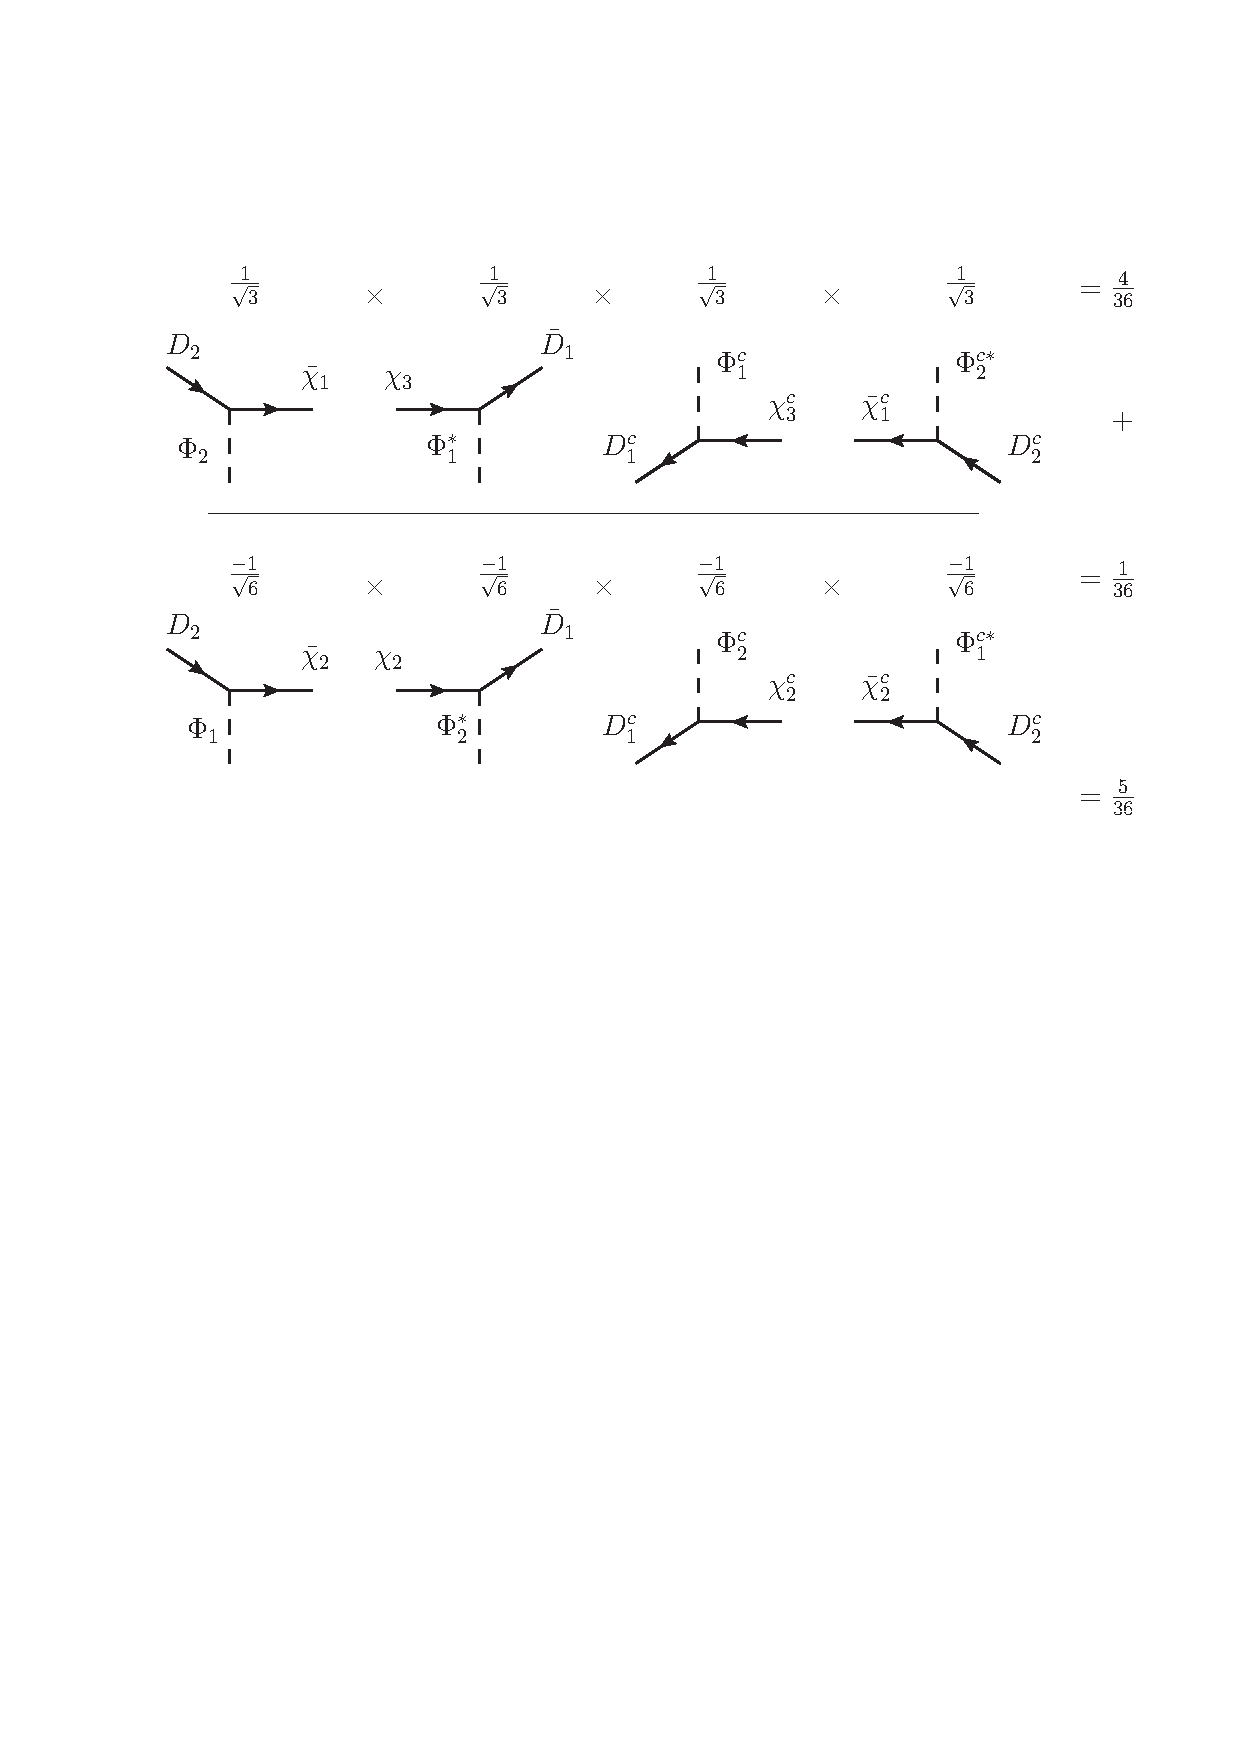
\includegraphics[width=1.2\textwidth]{CG.png}
 \caption{Three contributing diagrams for $dd\rightarrow ll$. Since you integrate over all internal momenta, the signs of the electic charges which are given
 within the box aren't known. The roman numers represent the component of the respective multiplet}
 \label{pic_CG}
\end{figure}
The upper left box looks like $D_2\Phi_3\Psi_1$ for the first roman numbers which gives compared to \eqref{eq_CGSU2singlet}  $-\frac{1}{2\sqrt{3}}$. 
As the inner momentum changes its sign during the integration, the inner particles becoming their charged conjugates which have due to the change of their
hypercharges another sign and order with respect to the charged components. The second roman numbers represent them and they give the same Clebsch Gordan
coefficient. Since we have four vertices, the number I will keep is $-\frac{1}{2\sqrt{3}}^4$. The upper right with the same argumentation yields a CG-coefficient
of $\frac{\sqrt{2}}{2\sqrt{3}}^4$ and the middle one $-\frac{1}{2}^4$. Now we add them up and get $\frac{7}{72}$ but we wanted $1+\frac59 = \frac{14}{9}$.
The factor between these two results is 16 which I still don't have an reason for. \textbf{But to me it looks like the right way to get this prefactor}.
That means that at least for our model A, the second term does not occur since we have no charged currents and all other processes are equal by means 
that they have the same CG-coefficients at each vertex. To get the 5/9 and the Pauli-term right was my main task the last two weeks. \textbf{If you want to, we
can talk about these things next week.}

\newpage
\begin{table}[ht]
 \begin{tabular}{c|c|c|c}
  Field & $SU(3)_C\times SU(2)_L\times U(1)_{Y_W}$ & $A_4 \times U(1)_\text{FN} \times Z_3$ & $U(1)_\chi$\\
  \hline
  $Q^i_L$ & (3,2,$\frac16$) & (1,$a^i$,$\omega$) & 0\\
  $U^i_R$ & (3,1,$\frac23$) & (1,$b^i$,$\omega^2$)& 0\\
  $D^i_R$ & (3,1,$-\frac13$) & (1,$c^i$,$\omega^2$)& 0\\
  $L^i_L$ & (1,2,$-\frac12$) & (3,0,$\omega$)& 0\\
  $E^i_R$ & (1,1,$-1$) & ($1 {^(} {'} {^,} '' {^)} $,$d^i$,$\omega^2$)& 0\\
  $\Phi_H$ & (1,2,$\frac12$) & (1,0,1)& 0\\
  \hline
  $\psi$ & (1,3,1) & (1,0,$\omega^2$)& 1\\
  $\Phi_l$ & (1,2,-$\frac12$) & ($1''$,0,1)& 1\\
  $\Phi_q$ & (3,2,-$\frac76$) & ($1$,0,1)& 1\\
  \hline
  $\Phi_T$ & (1,1,0) & ($3$,0,1)& 0\\

 \end{tabular}
\caption{Model B: Transformation rules for our SM and BSM fields. The index $i$ stands for the three generations which influence the charges under the 
$U(1)_\text{FN}$ $a-d$. The representation for $E_R$ also depends on the generation ($e^c \sim 1$, $\mu \sim 1''$, $\tau \sim 1'$).}
\label{tab_modelb}
\end{table}
\noindent Now I transfered the idea to our model B \ref{tab_modelb} and build at first the CG-term:
\begin{align}
 2\times2\times3 \subset 1 = \frac{1}{\sqrt{3}}\left(D_1\Phi_1\psi_3 - \frac{1}{\sqrt{2}}\left(D_1\Phi_2+D_2\Phi_1 \right)\psi_2 + D_2\Phi_2\psi_1 \right).
\end{align}
I thought a $Y_\psi = +1$ is nicer, since it is easier to identify the respective $SU(2)$-component due to their absolute charge and the electrically uncharged
one is the third component. In this case I got 10 diagrams in total: for $dd\rightarrow ll$, $du\rightarrow l\nu$, $ud\rightarrow \nu l$ and $uu\rightarrow \nu\nu$
two each and for $dd\rightarrow \nu\nu$ and $uu\rightarrow ll$ one each (the first fermion has each a bar above). The prefactors I get out of this with the same idea are: 
$\frac{5}{36}, \frac{4}{36}, \frac{1}{36}$ which have the same problem as in the former case, so I multiplied them by 12 so that they fit the following rules
\begin{align}
 1+X=C\frac{5}{36}\\
 1-X=C\frac{1}{36}\\
 2\cdot X = C\frac{4}{36}
\end{align}
These rules come out of \eqref{eq_effLag} if you expand the whole $\tau$-stuff. $X$ is the fraction I'm looking for, which is $\frac59$ in Gripaios case.
The factor $C$ is so far not motivated but has to be introduced to fit these rules. It was 16 in Gripaios case and 12 in mine. This means that my $X$ is
$\frac23$. Heureka. 
\begin{align}
 \mathcal{L}_\text{eff} \supset \frac{K(x_q,x_l)}{m^2}\frac{\alpha_i^{q*} \alpha_j^{q*} \alpha_m^l \alpha_n^l}{64\pi^2}\left[\left(\bar Q^i_L\gamma^\mu Q^j_L\right)\left(L^m_L\gamma_\mu L^n_L\right)+\frac23\left(\bar Q^i_L\gamma^\mu \vec \tau Q^j_L\right)\left(L^m_L\gamma_\mu \vec \tau L^n_L\right)\right].
 \label{eq_effLagMine}
\end{align}
I had two write this one down after all this work. 
At first I thought $C$ is the total number of processes. In Gripaios paper thats true. In the same order of processes as above, he has
for the first four ones 3 possible processes and the last two only two each which gives 16. So I'm afraid this would have just been too easy and it somehow
follows from another group theoretical consideration. But another
thing occured to me, which is a bit funny. Let's say we'd have a model wherein $Y_\psi=0$ as one could easily expect and therefore $Y_{\Phi_q} = -\frac16$ and
$Y_{\Phi_l}= +\frac12$. The processes as $dd\rightarrow \nu\nu$ have two diagrams now. I will sketch the origin. In the $Y_\psi = 1$ case we assign the 
scalars as $|Q(\Phi_q)|=\frac53$ and as a result $|Q(\Phi_l)|$ should be 2, but this doesn't exist. In the $Y_\psi = 0$ case we have $|Q(\Phi_q)|=\frac13$
which leads to $|Q(\Phi_l)|=0$ and $|Q(\Phi_q)|=\frac23$ to $|Q(\Phi_l)|=1$ which are both possible. I checked on the $SU(2)$-invariance at each vertex but
they all are allowed. So basically the question here is: \textbf{May a change in Hypercharge really have an influence on the amount of processes which are
$SU(2)$-invariant?} Well this would actually lead to 12 diagrams but the prefactor for the respective process would also change, so no real progress...

\subsection{$\bar B_s B_s$ - mixing}
\subsection{DM-annihilation $\bar \psi\psi \rightarrow \bar f f$ }



\newpage
\end{spacing}
\newpage
\begin{thebibliography}{xxx}
 \bibitem[1]{Grip}B. Gripaios et al. \textit{Linear flavour violation and anomalies in $B$ physics}\\ \href{http://arxiv.org/abs/1509.05020v1}{arxiv.org/abs/1509.05020v1}
 \bibitem[2]{Peskin}M. Peskin et al. \textit{An Introduction To Quantum Field Theory}\\ ISBN: 0-201-50397-2
 \bibitem[3]{Fierz}J.F. Nieves et al. \textit{Generalized Fierz identities}\\ \href{http://http://arxiv.org/abs/hep-ph/0306087v1}{arxiv.org/abs/hep-ph/0306087v1}
\end{thebibliography}
\end{document}
